\newpage
\section{Auswertung}
\subsection{Charakteristik Geiger-Müller-Zählrohrs}
Mit einer Integrationszeit von $60$s wird nun die gemessene Intensität
$N$ gegen die Betriebspanunngun $U$ aufgetragen.
Die gemessenen Impulse $N$ sind Poisson verteilt, sodass der Fehler
\begin{equation*}
    \Delta N = \sqrt{N},
\end{equation*}
folgt.
\begin{figure}
    \centering
    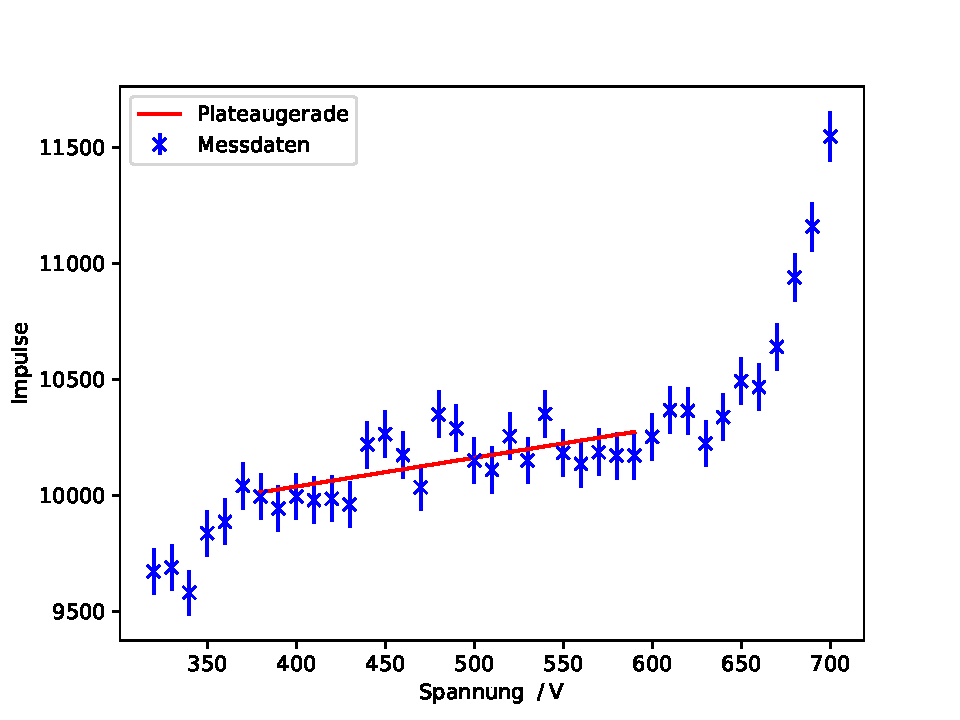
\includegraphics[width=0.7\textwidth]{input/p_charakteristik.pdf}
    \caption{Dargestellt sind die Impulse $N$ gegen die Betriebsspannung $U$ aufgetragen.
    Die lineare Ausgleichsgerade, liegt im Plateaubereich bei einer Spannung von
    380V - 590V.}
\end{figure}
\label{sec:Auswertung}
Für die Ausgleichsgerade des Plateaubereichs mit der Geradengleichung
\begin{equation}
    N=m\cdot U+n,
\end{equation}
ergeben sich die Parameter
\begin{align*}
    \text{Steigung m} &= (1.2\pm0.4)\frac{1}{\si{V}},\\
    \text{y-Abschnitt n}&= (9540\pm180).\\
\end{align*}

Für die Güte des Geiger-Müller-Zählrohrs ergibt sich aus der Steigung des
Plateaubereichs die Steigung M in \% pro $100$ V
\begin{equation*}
    M=1-\frac{m\cdot 400\text{V}+b}{m\cdot 500\text{V}+b}=(1.2\pm 0.35)\% \text{ pro } 100 \text{ V}.
\end{equation*}

\subsection{Bestimmung der Totzeit}
\subsubsection*{Zwei Quellen-Methode}
Für die zwei Quellen Methode ergeben sich die Impulsraten mit dn Poisson Fehlern und
der Integrationszeit von $120$s
\begin{align*}
    N_1=\frac{96941\pm310}{120\si{s}} && N_2=\frac{765180\pm277}{120\si{s}} && N_{1+2}=\frac{158479\pm398}{120\si{s}},
\end{align*} 
ergibt sich durch Gl. \ref{eqn:2Quellen} die Totzeit
\begin{equation}
    T \approx (115\pm4)\si{ns},
\end{equation}
mit dem Fehler
\begin{equation*}
    \Delta T = \sqrt{\left(\frac{N_{1+2}-N_1}{2N_1N_2^2}\cdot \Delta N_2\right)^2+\left(\frac{N_{1+2}-N_2}{2N_1^2N_2}\cdot \Delta N_1\right)^2+\left(-\frac{1}{2N_1N_2}\cdot \Delta N_{1+2}\right)^2}
\end{equation*}
\subsubsection*{Oszilloskop Methode}
Ließt man nun die Zeit zwischen dem ersten (der helle Peak) und zweiten Impuls ab, so 
entspricht der Abstand etwa einem Kästchen. Somit ist die Totzeit
\begin{equation*}
    T\approx 100\mu s
\end{equation*}
\begin{figure}
    \centering
    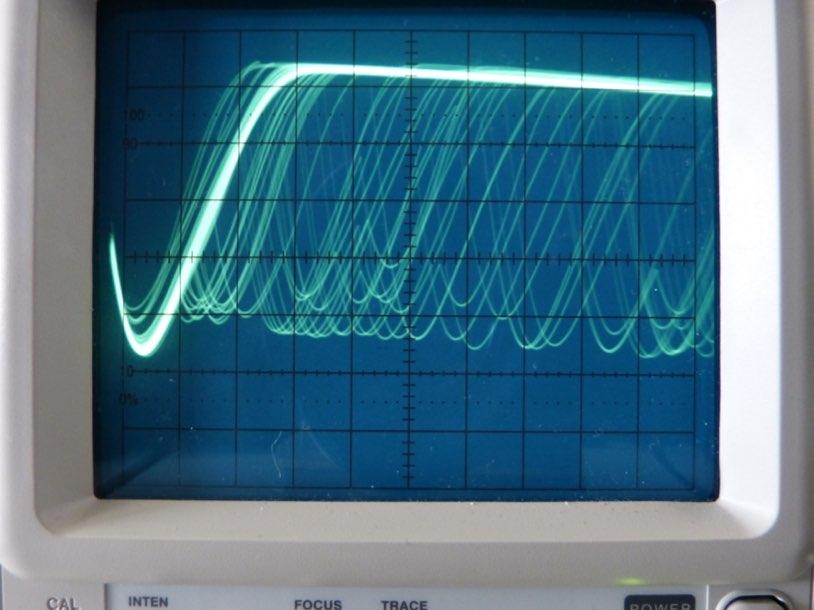
\includegraphics[width=0.7\textwidth]{input/oszilloskop.jpg}
    \caption{Oszilloskopbild aufgenommen mit einer Zeitachse von 100$\mu$s/DIV.}
\end{figure}
\subsection{Freigesetzte Ladungen}
Nach Gl. \ref{eqn:strom} lassen sich die pro einfallendem teilchen freigesetzten Ladungen
berechnen. Für den Fehler folgt
\begin{equation*}
    Z=\sqrt{\left(\frac{1}{eN} \cdot \Delta I\right)^2+\left(\frac{1}{eN^2} \cdot \Delta N\right)^2}.
\end{equation*}
Somit ergibt sich
\begin{table}
    \centering
    \begin{tabular}{c c c}
        \toprule
        $I\;/\;$nA & Impulsrate $\;/\;\frac{1}{s}$ & $Z\;/\;e\cdot 10^{10}$\\
        \midrule
        300\pm 50  & 163.9\pm 1.7 & 1.14\pm 0.19 \\
        400\pm 50  & 166.6\pm 1.7 & 1.50\pm 0.19 \\
        700\pm 50  & 171.1\pm 1.7 & 2.55\pm 0.18 \\
        800\pm 50  & 169.2\pm 1.7 & 2.95\pm 0.19 \\
        1000\pm 50 & 169.7\pm 1.7 & 3.68\pm 0.19 \\
        1030\pm 50 & 170.9\pm 1.7 & 4.75\pm 0.19 \\
        1040\pm 50 & 174.9\pm 1.7 & 5.00\pm 0.18 \\
        1080\pm 50 & 192.4\pm 1.8 & 5.84\pm 0.17 \\
        \bottomrule
    \end{tabular}
    \caption{Die Tabelle zeigt die Anodenströme, Implsraten und den daraus resultierden
    freigesetzten Ladungen pro einfallendem Teilchen.}
    \label{tab:tabelle}
\end{table}
\begin{figure}
    \centering
    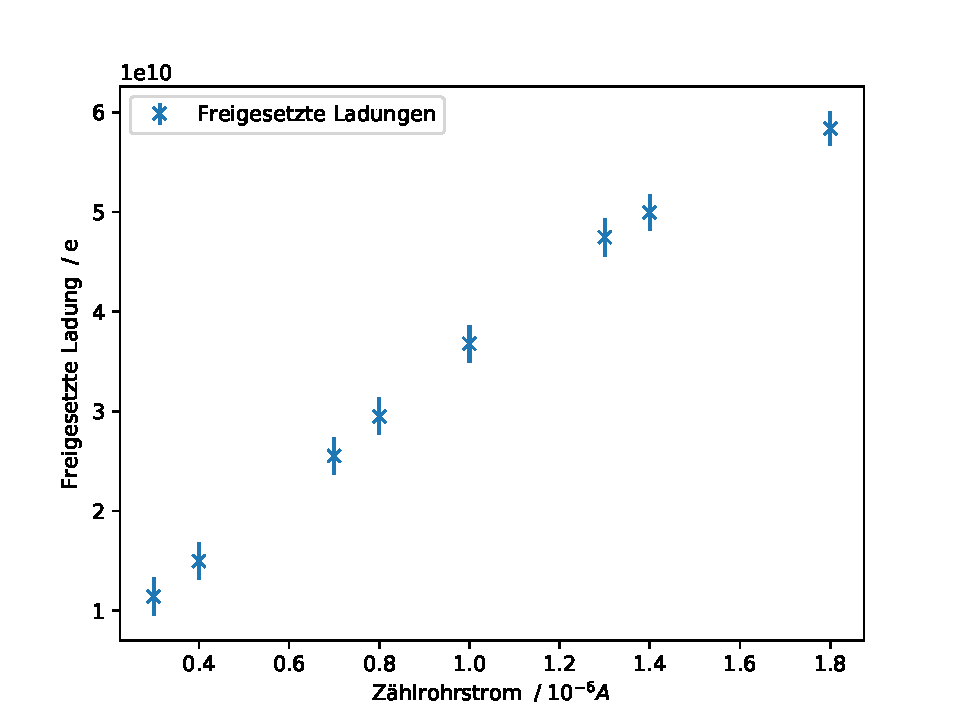
\includegraphics[width=0.7\textwidth]{input/Ladungen.pdf}
    \caption{Dargestellt ist die freigesetzte Ladgung gegen den Zählrohrstrom aufgetragen.}
\end{figure}